\documentclass{beamer}
\usetheme{Boadilla}
\usepackage{graphicx}


\title{Rinnakkaisuus verkkopalvelinsovelluksessa}
\author{Vili Lipo}
\institute{Helsingin Yliopisto}
\date{\today}

\begin{document}
\begin{frame}
\titlepage
\end{frame}
\begin{frame}
\frametitle{Esityksen rakenne}
\tableofcontents
\end{frame}
\section{Johdanto}
\begin{frame}
\frametitle{Johdanto}
\begin{itemize}
 \item Selvittää minkälaista rinnakkaisuus on verkkopalvelinsovelluksessa
 \item Tutkielman tarkoitus oli selvittää miksi tapahtumavetoiset palvelimet
 ovat niin suosittuja (Node.js).
 \item Perehtyä niiden vahvuuksiin ja heikkouksiin
 \end{itemize}
\end{frame}
\section{Verkkopalvelinsovellus}
\subsection{Asiakas-palvelin malli}
\begin{frame}
    \frametitle{Asiakas-palvelin malli}
    \begin{itemize}
        \item Asiakasosa tarjoaa käyttöliittymän
        \begin{itemize}
            \item työpöytäohjelma
            \item verkkosivu
            \item komentoriviohjelma
        \end{itemize}
        \item Palvelin tarjoaa palveluita verkkoyhteyden yli
            \begin{itemize}
                \item Tiedostoja
                \item Laskentaa
                \item Dataa
                \item Useille asiakkaille samanaikaisesti
            \end{itemize}
    \end{itemize}
\end{frame}
\begin{frame}
    \frametitle{Verkkopalvelinsovellus}
    \begin{itemize}
        \item Verkkopalvelinsovellus vastaa internetin selaamiseen liittyviin pyyntöihin.
        \item HTTP-pyynnöt
            \begin{itemize}
                \item GET
                \item POST
                \item DELETE
                \item etc..
            \end{itemize}
        \item Lähettää ja vastaanottaa tekstimuotoista dataa.
        \item I/O-sidonnainen sovellus
    \end{itemize}
\end{frame}
\subsection{Rinnakkaisuus}
\begin{frame}
    \frametitle{Rinnakkaisuus}
    \begin{itemize}
       \item Operaatioiden suorittamista samaan aikaan laitteistoa hyödyntäen
        \begin{itemize}
            \item Useita suorittimia yhdellä sirulla
        \end{itemize}
        \item Ongelmakohtaista
            \begin{itemize}
                \item Peräkkäisyys
                \item Ahmdalin laki \\
                    \[ S_{\text{latency}}(s) =  \frac{1}{(1-p) + \frac{p}{s}} \]
                    Määrää teoreettisen maksimin rinnakkaistamalla
                    saatavalle nopeutukselle.
            \end{itemize}
        \item Ongelmallista
            \begin{itemize}
                \item Lukkiutuminen
                \item Kilpailutilanteet
            \end{itemize}
    \end{itemize}
\end{frame}

\begin{frame}
    \frametitle{Prosessit ja Säikeet}
    \begin{itemize}
        \item Käyttöjärjestelmä hallinnoi prosesseja, joita
            voi olla useita ajossa samaan aikaan
        \item Prosessin suoritus voi olla yhdessä tai useammassa säikeessä
        \item Tässä esitelmässä keskitytään ytimen tason säikeisiin
            \begin{itemize}
                \item Aikatauluttamisesta vastaa käyttöjärjestelmä
                \item Useita voi olla aikaan ajossa
                \item Voidaan hyödyntää sovelluksen rinnakkaistamiseen
            \end{itemize} 
    \end{itemize}

\end{frame}


\begin{frame}
    \frametitle{Asynkroniset operaatiot}
    \begin{itemize}
        \item Menetelmä jolla voidaan suorittaa I/O-operaatioita rinnakkain
            luomatta uusia säikeitä ohjelmalle.
        \item I/O-operaatioiden siirtämistä käyttöjärjestelmän
            suoritettavaksi
        \item Kutsuva prosessi/säie ei jää odottamaan valmistumista,
            ja jatkaa suoritustaan
        \item Voi aiheuttaa kilpailutilanteita
        \item Tehostaa I/O-resurssien hyödyntämistä
    \end{itemize}
\end{frame}
\section{Rinnakkaistamismalleja}
\subsection{Moniprosessiset ja monisäikeiset mallit}
\begin{frame}
    \frametitle{Moniprosessiset ja monisäikeiset mallit}
    \begin{itemize}
        \item Säie-pyyntöä-kohti-malli
        \item Säireservimalli (threadpool-model)
    \end{itemize}
\end{frame}
\begin{frame}
    \frametitle{Säie-pyyntöä-kohti-malli (OTPR)}
    \begin{itemize}
        \item Luonteva tapa rinnakkaistaa palvelimen toimintaa
        \item Jokaista asiakkaan pyyntöä kohti luodaan uusi säie
        \item Säie käsittelee pyynnön
        \item Säie tuhotaan
        \item Ongelma: luominen ja tuhoaminen kallista
            \begin{itemize}
                \item Ratkaisu: Säiereservimalli
            \end{itemize}
    \end{itemize}
\end{frame}
\begin{frame}
    \frametitle{Säiereservimalli}
    \begin{itemize}
        \item Luodaan valmiiksi reserviin tietty määrä säikeitä
        \item Asiakkaan pyyntö osoitetaan vapaalle säikeele
        \item Tapahtuman käsittelyn jälkeen säie palautetaan reserviin
        \item Säikeiden luomiseen ja tuhoamiseen ei kulu aikaa
    \end{itemize}
\end{frame}
\subsection{Tapahtumaohjatut mallit}
\begin{frame}
    \frametitle{Tapahtumaohjatut mallit}
    Tapahtumaohjatut mallit ovat olleet käytössä pitkään
    muun muassa käyttöliittymäohjelmoinnissa.
    Soveltuvat mielekkäästi palvelimiin, sillä
    pyynnöt kuvautuvat hyvin tapahtumiksi.\\
    Malleja:
    \begin{itemize}
        \item Reactor
        \item Proactor
        \item SEDA
    \end{itemize}
\end{frame}
\begin{frame}
    \frametitle{Reactor}
    \begin{itemize}
        \item Yleinen tapahtumaohjattu synkroninen malli
        \item Soveltuu kevyen taakkojen palvelimiin
        \item Mekanismi jolla voidaan odottaa pyyntöjä useista lähteistä
        \item I/O-operaatiot suoritetaan, kun resurssi on vapaa.
    \end{itemize}
\end{frame}
\begin{frame}
    \frametitle{Esimerkki: Pyynnön käsittely Reactor-mallissa}
        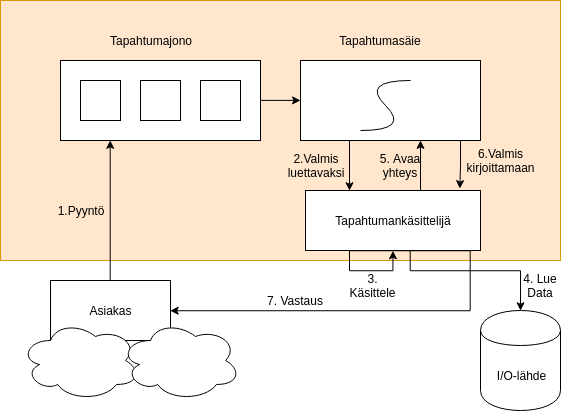
\includegraphics[scale=0.5]{reactor.png}
\end{frame}
\begin{frame}
    \frametitle{Proactor}
    \begin{itemize}
        \item Tapahtumaohjattu asynkroninen malli
        \item Reactor-mallista osaa käytetään asynkronisten
            operaatioiden valmistumisten hallintaan
        \item Mahdollistaa asynkronisten operaatioiden ketjuttamisen
        \item Käyttöjärjestelmälle määritellään millaista tapahtumaa
            odotetaan ja mikä käsittelijä tapahtumasta vastaa
            \begin{itemize}
                \item Vastakutsu (callback)
            \end{itemize}
        \item Käyttöjärjestelmä ilmoittaa kun I/O-operaatio on valmis
    \end{itemize}
\end{frame}
\begin{frame}
    \frametitle{Esimerkki: Pyynnön käsittely Proactor-mallissa}
        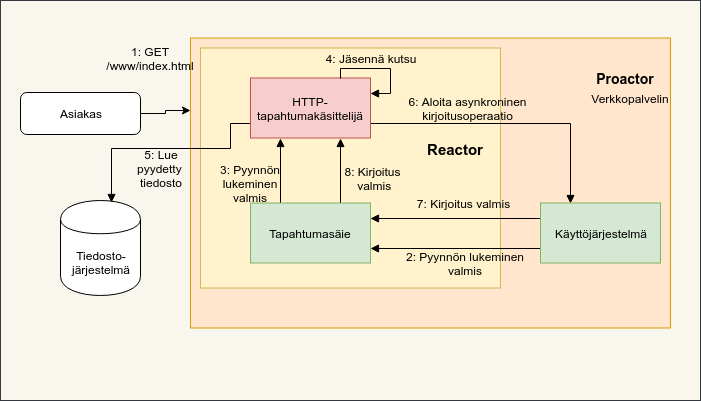
\includegraphics[scale=0.5]{Proactor.png}
\end{frame}
\begin{frame}
    \frametitle{Staged event driven architecture}
    \begin{itemize}
        \item Tapahtumakäsittelijät jaettu tasoille
        \item Jokaisella tasolla työntekijäsäikeitä
        \item Rajataan rinnakkaistaminen tasokohtaiseksi
        \item Yleinen pilvilaskennassa
    \end{itemize}
\end{frame}
\section{Vertailu}
\subsection{Kriteerit}
\begin{frame}
    \frametitle{Vertailu: Kriteerit}
    \begin{enumerate}
        \item Suorituskyky ja Skaalautuvuus
            \begin{enumerate}
                \item Volyymi
                \item Viive
                \item Menetysprosentti
            \end{enumerate}
        \item Sovelluslogiikan kehitystyön haastavuus
        \item Vakaus
    \end{enumerate}
\end{frame}
\subsection{Suorituskyky}
\begin{frame}
    \frametitle{Suorituskyky ja Skaalautuvuus}
    \begin{itemize}
        \item Ei selkeää voittajaa
        \item Verkkopalvelin on I/O-sidonnainen sovellus
            \begin{itemize}
                \item Tiedostojen lähettämistä ja vastaanottamista 
                \item Asynkronisilla kutsuilla samanaikaistamisen
                    voi siirtää käyttöjärjestelmän vastuulle
                \item Edut korostuu suurilla tiedostoilla
            \end{itemize}
        \item Säikeiden käsittelyyn kuluva aika
            \begin{itemize}
                \item Kontekstinvaihdot aiheuttavat huomattavaa viivettä
                    SEDA-mallissa
                \item Säiereservimallissa tulee kiinnittää huomiota reservin kokoon
            \end{itemize}
    \end{itemize}
\end{frame}
\subsection{Sovelluslogiikan kehitystyön haastavuus}
\begin{frame}
    \frametitle{Sovelluslogiikan kehitystyön haastavuus}
    \begin{columns}
        \column{0.5 \textwidth}
        \textbf{Proactor/Reactor}
            \begin{itemize}
                \item Pyynnön käsittelyajan tulee olla lyhyt
                    \begin{itemize}
                        \item Muu ohjelma odottaa yksittäisen pyynnön valmistumista
                    \end{itemize}
                \item Asynkroniset I/O-operaatiot
                    \begin{itemize}
                        \item Käyttö haastavaa
                        \item Ajoitus
                        \item Vastakutsujen käyttö
                            \begin{itemize}
                                \item Abstraktioita: Promise, Future, async/await
                            \end{itemize}
                    \end{itemize}
                \item Sovelluksen kulun seuraaminen on vaikeaa
            \end{itemize}
        \column{0.5 \textwidth}
        \textbf{Säiereservimalli}
            \begin{itemize}
                \item Ei aseta suuria rajoitteita sovelluslogiikalle
                \item Pitkäkestoinen laskenta estää vain laskentaa koskevan säikeen
                    \begin{itemize}
                        \item Muiden pyyntöjen suoritus jatkuu muilla säikeillä
                    \end{itemize}
                \item Mahdolliset lukkiutumiset
                \item Kilpailutilanteet
            \end{itemize}
    \end{columns}
\end{frame}
\subsection{Vakaus}
\begin{frame}
    \frametitle{Vakaus: ReDOS-hyökkäys}
    \begin{itemize}
        \item Regular Expression Denial Of Service
        \item Palvelunestohyökkäyksen alaluokka
        \item Kohdistuu pyynön polun jäsentävään osaan
            \begin{itemize}
                \item Tapahtumaohjatuissa palvelimissa estää koko sovelluksen kulun
                \item Monisäikeisissä yhden säikeen kerrallaan
            \end{itemize}
        \item Tehokkuus perustuu vaikeasti ratkaistavaan säännölliseen lauseeseen
            osoitepolussa
        \item Tarvittavien pyyntöjen määrä paljon pienempi kuin tavallisessa
            DOS-hyökkäyksessä, jos kohteena tapahtumaohjattu palvelin
        \item Suojautua voi aikarajoittamalla polun jäsentämiseen kuluvan 
            ajan
    \end{itemize}
\end{frame}
\section{Yhteenveto}
\begin{frame}
    \frametitle{Yhteenveto}
    \begin{itemize}
        \item Verkkopalvelinsovellus on I/O-sidonnainen
        \item I/O:ta voi suorittaa rinnakkain usealla säikeellä,
            tai asynkronisilla operaatioilla
        \item Asynkroniset kutsut yhdistettynä tapahtumaohjattuun
            ohjelmointiin luovat hyvän työkalupakin kehittäjälle
        \item Säikeiden tai prosessien käyttöä vaaditaan
            laskennan rinnakkaistamiseen
    \end{itemize}
\end{frame}
\end{document}
